\documentclass[12pt,letterpaper]{article}


\usepackage{amsmath}
\usepackage{amsfonts}
\usepackage{amsthm}
\usepackage{amssymb}
\usepackage{ulem}
\usepackage{tikz}
\usepackage{pgfplots}
\pgfplotsset{compat=1.8}


\newcommand\mybox[2][]{\tikz[overlay]\node[fill=yellow!20,draw=black,inner sep=2pt, anchor=text, rectangle, rounded corners=1mm,#1] {#2};\phantom{#2}}
\usepackage{graphicx}

\newcommand{\Lim}[1]{\raisebox{0.5ex}{\scalebox{0.8}{$\displaystyle \lim_{#1}\;$}}}


\title{Mandatory Assignment 1 of 2}
\author{Håkon Berggren Olsen\\
  \small{MAT2400- Real Analysis}\\
  \small{University of Oslo}\\
  \small{hakonberggren@gmail.com}
}
\date{Spring 2022}

\begin{document}
\maketitle
\newpage 
 
\section*{Problem 1}
 
 Let $X$ be the set of all sequences $\{x_n\}_{n\in \mathbb{N}}$ of real numbers such that $\lim_{n\to \infty} x_n = 0$.\\
 \noindent \\
 a) Use the definiton of convergence to show that if $\{x_n\}\in X$, then there is a $K\in \mathbb{N}$ such that $|x_K|=\text{sup}\{|x_n| : n\in \mathbb{N} \}$ (i.e. $x_K$ is an element of maximal absolute value).\\
 
\noindent\fbox{
    \parbox{\textwidth}{
 \noindent \\
 As all sequences $\{x_n\}_{n\in \mathbb{N}}$ in $X$ converges to $0$, $lim_{n\to \infty} x_n = 0$, the defintion of convergence states:

For every $\epsilon>0$ there exists a $N\in \mathbb{N}$ such that 
\begin{align*}
	|x_n-0| = |x_n|<\epsilon
 \end{align*}
%  \noindent
% \textbf{Definition of convergence:}\\
 %''A sequence $\{x_n\}$ of real numbers converges to $a\in\mathbb{R}$ if for every $\epsilon >0$ (no matter how small), there is an $N\in\mathbb{N}$ such that $|x_n-a|<"\epsilon$ for all $n\le N$. We write $lim_{n \to \infty} x_n = a$.''\\
 
%Pointers from lecturer:\\
% Think of a sequence as a point in a space, i.e. $\{x_n\}$ is a point in the space of $X$. \\

\noindent 

As the series converges, one can choose an $\epsilon>0$ such that there exists an $N\in\mathbb{N}$ where $|x_n|$ is no longer increasing. Therefore there must exists a $K\in\mathbb{N}$ such that $K\le N$ where 
 \begin{align*}
 	|x_K| = \text{sup} \{|x_n| \ : | n\in\mathbb{N}   \}
 \end{align*}
 

\textbf{Note:} This is a very wordy argument and I am not quite sure how to phrase it more rigorously.
 
    }
}


 
%All sequences in $X$ are real numbers and converges to $0$ and are therefore Cauchy sequences (Theorem 2.2.5 in \cite{lindstrom2017}, ''Completenes of $\mathbb{R}^m$ '' and Propostiion 2.2.6), and every Cauchy sequence in $\mathbb{R}$ is bounded. 
 
 


\newpage
 \noindent \\
 b) Define $d: X \times X \to [0, \infty)$ by
\begin{align*}
 	d(\{x_n\}, \{y_n\}) = \text{sup}\{|x_n-y_n| : n\in \mathbb{N}\}. 
\end{align*}
 Show that d is a metric on $X$.\\
 \noindent \\


\noindent\fbox{
    \parbox{\textwidth}{


For $(X,d)$ to be a metric space, it needs to satisfy the properties of postivity, symmetry and the triangle inequality:
 \begin{itemize}
 	\item (Positivity) For all $x,y\in X$, we have $d(x,y)\ge 0$ with equalitiy if and only if $x=y$.
 	\item (Symmetry) For all $x,y \in X$ we have $d(x,y)=d(y,x)$. 
 	\item (Triangle Inequality) For all $x,y,z \in X$, we have
 		\begin{align*}
 			d(x,y) \le d(x,z)+d(z,y)
 		\end{align*}
 \end{itemize}

The first two properties are fairly obvious as $|x_n-y_n|\ge 0$ (postivity) and $|x_n-y_n| = |y_n-x_n|$ (symmetry). To prove the triangle inequality, first assume there exists $\{x_n\},\{y_n\},\{z_n\}\in X$. Looking at the argument for the supreme function we have the triangle inequality
\begin{align*}
	|x_n-y_n| &\le |x_n-z_n| + |y_n - z_n|
\end{align*}
further evaluating the supremum
\begin{align*}
	|x_n-z_n| + |y_n - z_n| &\le  \text{sup} \{|x_n-z_n| + |y_n - z_n|  : n\in\mathbb{N} \} \\
		&\le \text{sup} \{|x_n-z_n| : n\in\mathbb{N} \} +\text{sup} \{| z_n-y_n|  : n\in\mathbb{N} \} \\
		&= d(\{x_n\}, \{z_n\}) + d(\{z_n\}, \{y_n\})
\end{align*}
where the fact that $\text{sup} \{A+B\} = \text{sup} \{A\} + \text{sup} \{B\}$ is used. \\
This results in $d(\{x_n\}, \{z_n\}) + d(\{z_n\}, \{y_n\})$ being an upper bound \footnote{Not the least upper bound, hence the inequality.} for $|x_n-y_n|$ and we therefore get

 \begin{align*}
	 d(\{x_n\}, \{y_n\}) \le d(\{x_n\}, \{z_n\}) + d(\{z_n\}, \{y_n\})
\end{align*}
    }
}

 \noindent \\
 c)  Let $Y$ be the set of all sequences $ \{y_n\}_{n\in\mathbb{N}}$ of real numbers such that $\sum_{n=1}^{\infty} |y_n| < \infty$. Show that $Y \subseteq X$. Find a sequence $\{x_n\}$ that belongs to $X$ but not to $Y$ (you can use everything you know from calculus).\\
 
\noindent\fbox{
    \parbox{\textwidth}{

 
 We have 
 \begin{align*}
 	X &= \{ \{x_n\} \ | \ \lim_{n\to\infty} x_n = 0, n\in\mathbb{N}\} \\
	Y &= \{ \{y_n\} \ | \ \sum_{n=0}^{\infty}|y_n|<\infty, n\in\mathbb{N}\} 
 \end{align*}
 
 Define $S_N = \sum_{n=0}^N |y_n|$, which converges as it is smaller than infinity. We can then write
 \begin{align*}
 	\text{lim}_{n\to\infty} \left( S_N - S_{N-1}\right) = L-L = 0
 \end{align*}
 
 but
 
 \begin{align*}
 	S_N - S_{N-1} &= \left( |y_0| + |y_1| + \cdot \cdot \cdot |y_N|\right) - \left( |y_0| + |y_1| + \cdot \cdot \cdot |y_{N-1}|\right) \\
 	&= |y_n|
 \end{align*}
 So we have that $|y_N|=0$ and therefore all sequences in $Y$ converges to $0$ and therefore $Y \subseteq X$.
 
 
 \noindent
 A sequence $\{x_n\}$ that belongs to $X$ but not to $Y$ is the harmonic series, $\frac{1}{n}$. This series converges to zero as $\lim_{n \to \infty} 1/n = 0$, but the sum of the absolute value of the sequence is not smaller than infinity.
\begin{align*}
	\sum_{n=1}^\infty \left| \frac{1}{n}\right |  \nless \infty
\end{align*} 

    }
}
\newpage

 \noindent \\
d) Assume $\{x_n\} \in X \backslash Y$ and let $\epsilon > 0$. Show that the ball $B(\{x_n\}; \epsilon)$ contains elements from $Y$. Explain why this shows that  $Y$ is not closed.\\
 

\noindent\fbox{
    \parbox{\textwidth}{

Assuming $\{x_n\} \in X \backslash Y$ means we are looking at the sets $\{x_n\}$ which have the following properties
\begin{align*}
	\lim_{x\to\infty} \{x_n\} = 0 \quad \text{and} \quad \sum_{n=1}^\infty |x_n| &= \infty
\end{align*}

We need to prove that the ball 
\begin{align*}
	B(\{x_n\}; \epsilon) = \{\{z_n\} \in X \backslash Y : \ d( \{z_n\}, \{x_n\})< \epsilon \}
\end{align*}
contains elements from $Y$: i.e. show that there exists a $\{z_n\}$ such that
\begin{align*}
	|z_n -x_n| < \epsilon
\end{align*}
for  $\sum_{n=1}^\infty |z_n| <0$.
We know that $\sum_{n=1}^\infty |z_n|$ converges if and only if $\sum_{n=N}^\infty |z_n|$ converges for all $N\in\mathbb{N}$. Considering 
\begin{align*}
	\{\widetilde{z_n}\} = \{ z_1, z_2, z_3, ..., z_n, 0, 0, ..., 0, ...\}
\end{align*}
which also converges as  $\sum_{n=N}^\infty |z_n|$ converges. Incorporating this we get
\begin{align*}
	|\widetilde{z_n}-x_n|\le  |z_n -x_n| <\epsilon \\
\end{align*}
Supposing $N$ is where the entries in the sequence $\{\widetilde{z_n}\}$ become zero, choosing an $n>N$ we get
\begin{align*}
	|\widetilde{z_n}-x_n| = |0-x_n|&\le  |z_n -x_n| <\epsilon \\
	|x_n|&< \epsilon
\end{align*}

Which is true as $lim_{n\to\infty} |x_n| =0$ converges and thus we can always find an $N$ far enough out such that this holds.

Since we have chosen the open ball, this means that $Y$ is not closed as [...].


%Tom: "What can you do to $\{x_n\}$ to make it converge without messing with the sequence \emph{too} much. "

%\noindent
%Erik: "A sum $\sum_{n=1}^\infty |x_n|$ converges if and only if $\sum_{n=N}^\infty |x_n|$ converges for each $N\in\mathbb{N}$. So summing up the "tail" of the sequence, starting from $N$, is the problem. We can get the tail $\{x_n\}$ as close to zero as we wish as $\lim_{n\to\infty} x_n = 0$. \\
%\noindent 
%Try to look at sequences where the tail is then removed, i.e.
%\begin{align*}
%	\{x_1, x_2, x_3, ..., x_N, 0,0,...,0,...\}
%\end{align*}
 




   }
}
\newpage
 
 \noindent \\
e) Assume $\{y_n\}\in Y$ and let $\epsilon >0$. Show that $B(\{y_n\};\epsilon)$ contains elements from $X \backslash Y$ Explain why this shows that $Y$ is not open. \\
 

\noindent\fbox{
    \parbox{\textwidth}{
Assuming $\{y_n\} \in Y $ means we are looking at the sets $\{y_n\}$ which have the following properties
\begin{align*}
	\lim_{x\to\infty} \{y_n\} = 0 \quad \text{and} \quad \sum_{n=1}^\infty |y_n| &< \infty
\end{align*}

We need to prove that the ball 
\begin{align*}
	B(\{y_n\}; \epsilon) = \{\{z_n\} \in Y : \ d( \{z_n\}, \{y_n\})< \epsilon \}
\end{align*}
contains elements from $X\backslash Y$: i.e. show that there exists a $\{z_n\}$ such that
\begin{align*}
	|z_n -y_n| < \epsilon
\end{align*}
for $\sum_{n=1}|y_n|<\infty$ and $\sum_{n=1}|z_n| = \infty$.

Following from the previous argument, consider a 
\begin{align*}
	\{\widetilde{y_n}\} = \{y_1, y_2, y_3, ..., y_n, 0, 0, ..., 0, ...\}
\end{align*}
which also converges as $\sum_{n=N} |y_n|$ convergers. By using the fact that $|z_n-y_n| = |y_n-z_n|$ we get 

\begin{align*}
	|y_n-z_n|  < \epsilon
\end{align*}
Supposing $N$ is where the entries in the sequence $\{\widetilde{y_n}\}$ become zero, choosing an $n>N$ we get

\begin{align*}
	|\widetilde{y_n} -z_n| = |0-z_n| &\le |y_n-z_n| < \epsilon\\
	|z_n| &< \epsilon
\end{align*}
Which is true as $lim_{n\to\infty} |z_n| =0$ converges and thus we can always find an $N$ far enough out such that this holds.


Since we have chosen the open ball, this means that $Y$ is not open as [...].

    }
}
\newpage

 
 
\section*{Problem 2}

A metric space $(X,d)$ is called disconnected if there are two non-empty, open subsets $O_1, O_2$ such that $O_1 \cup O_2 = X$ and $O_1 \cap O_2 = \emptyset$. \\
%DONE
\noindent \\
a) Let $X = [0,1] \cup [2,3]$ have the usual metric $d(x,y) = |x-y|$. Show that $(X,d)$ is disconnected. \\
\noindent \\


\noindent\fbox{
    \parbox{\textwidth}{
The metric space $(X,d)$ is composed of two closed sets. \\
By carefully splitting $X$ into $O_1= [0,\frac{1}{2}) \cup (\frac{3}{2},3]$ and $O_2 = (\frac{1}{2},1]\cup [2,\frac{3}{2})$, the ''inside'' and the ''outside'' of $X$, we now have two non-empty, open subsets which satisfy the properties of a disconnected metric space.
\begin{align*}
	O_1 \cup O_2  &= \left([0,\frac{1}{2}) \cup (\frac{3}{2},3]\right) \cup \left((\frac{1}{2},1]\cup [2,\frac{3}{2})\right)    = X \\
	O_1 \cap O_2  &= \left( [0,\frac{1}{2}) \cup (\frac{3}{2},3]\right) \cap \left( (\frac{1}{2},1]\cup [2,\frac{3}{2})\right)  = \emptyset
\end{align*}

    }
}




\noindent \\
b) Show that $\mathbb{Q}$ with the usual metric $d(x,y)=|x-y|$ is disconnected. \\
(Hint: Consider $O_1=\{x\in\mathbb{Q} : x^2 > 2\}$ and $O_2=\{x\in\mathbb{Q} : x^2 > 2\}$.)\\

\noindent\fbox{
    \parbox{\textwidth}{

\noindent \\
Considering $O_1=\{x\in\mathbb{Q} : x^2 > 2\}$ and $O_2=\{x\in\mathbb{Q} : x^2 < 2\}$, which are open, non-empty subsets of $\mathbb{Q}$. The metric space is disconnected as the subset are disjointed

\begin{align*}
	O_1 \cup O_2 = \{x\in\mathbb{Q} : x^2 > 2\}\cap\{x\in\mathbb{Q} : x^2 < 2\} = \mathbb{Q} \\
	O_1 \cap O_2 = \{x\in\mathbb{Q} : x^2 > 2\}\cup\{x\in\mathbb{Q} : x^2 < 2\} = \emptyset \\
\end{align*}
    }
}




\noindent \\
c) Assume that $(X,d)$ is a connected (i.e. not disconnected) metric space and that $f : X \to \mathbb{R}$ is a continous function such that there are two points $a,b \in X$ with $f(a)<0<f(b)$. Show that there is a point $c\in X$ such that $f(c)=0$.(This is an abstract version of the Intermediate Value Theorem.)




\noindent\fbox{
    \parbox{\textwidth}{
	To prove there exists a $c\in \mathbb{X}$ such that $f(c)=0$, we need to prove that given $(X,d)$ is connected we have $f(X)$ to be connected. Because if $f(X)$ is connected, the two sets $(a,c]$ and $[c,b)$ contradicts the defintion of disconnected sets
\begin{align*}
	O_1 \cap O_2 = (a,c] \cap [c,b) \neq \emptyset
\end{align*}
which means there must be a $c\in X$ such that $f(c)=0$. Under is the proof that given $(X,d)$ is connected and $f(X)$ is continous, then $f(X)$ is connected:\\
\textbf{Proof by the contrapositive}: \\
	Suppose $f:X\to F(X)$ is a surjective (?), continous function and that $f(X)$ is disconnected. Since $f(X)$ is disconnected, there must be two open subsets $U_1$ and $U_2$ in $f(X)$ such that 
\begin{align*}
	U_1 \cup U_2&= f(X)\\
	U_1 \cap U_2&= \emptyset
\end{align*}
Let $O_1 = f^{-1}(U_1)$ and $O_2 = f^{-1}(U_2)$, and as $U_1, U_2$ are open sets so are $O_1, O_2$. 
For every $x\in X$, the union of the two subsets are
\begin{align*}
	O_1 \cup O_2 = X
\end{align*}
because $f(x)$ is either in $U_1$ or $U_2$. Since $f(x)$ cannot be in both $U_1$ and $U_2$ since they are disconnected, we have that 
\begin{align*}
	O_1 \cap O_2 = \emptyset
\end{align*}
Thus $f(X)$ is disconnected.

% Tikz figure
\begin{center}
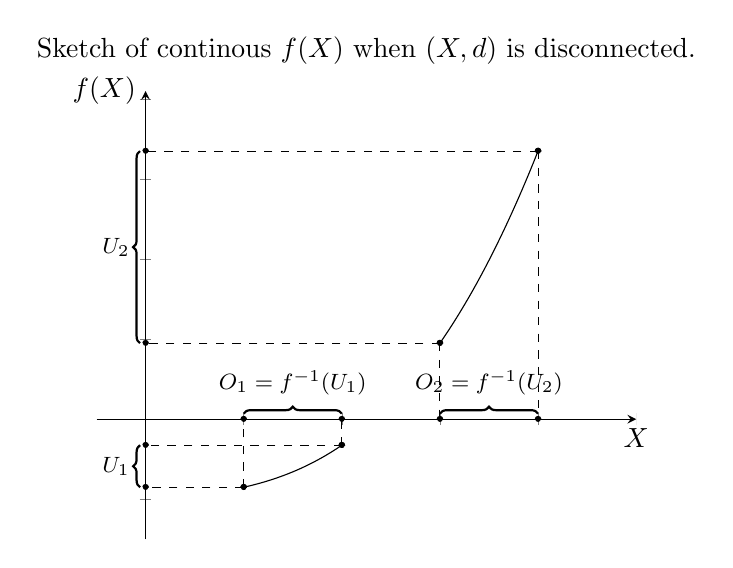
\begin{tikzpicture}
	\centering
	\begin{axis}[
	axis x line = middle,
	axis y line = middle,
	every axis x label/.style={at={(current axis.right of origin)},anchor=north},
      every axis y label/.style={at={(current axis.above origin)},anchor=east},
	ymin = -3,
	xmin = -0.25,
	ymax = 8.2,
	xmax = 2.5,
	xlabel=$X$,
	ylabel=$f(X)$, 
	yticklabels={,,},
	xticklabels={,,},
	enlargelimits=false,
	title={Sketch of continous $f(X)$ when $(X,d)$ is disconnected.},
	]	
	\addplot[black, domain=0.5:1]
		{x^3+20*sin(x)-2};	
	\addplot[black, domain=1.5:2]
		{x^3+20*sin(x)-2};

 	%Horizontal lines	
	\addplot[dashed, mark=*, mark options={scale=0.5}] coordinates {(0.5,	-1.70047) (0, -1.70047)};	
	\addplot[dashed, mark=*, mark options={scale=0.5}] coordinates {(1,		-0.65095) (0,-0.65095)};	
	\addplot[dashed, mark=*, mark options={scale=0.5}] coordinates {(1.5,	1.898539) (0,1.898539 	)};	
	\addplot[dashed, mark=*, mark options={scale=0.5}] coordinates {(2.0,	6.69799) (0,6.69799		)};	

	% Vertical lines	
	\addplot[dashed, mark=*, mark options={scale=0.5}] coordinates {(0.5,	-1.70047) (0.5, 0)};	
	\addplot[dashed, mark=*, mark options={scale=0.5}] coordinates {(1,		-0.65095) (1,0)};	
	\addplot[dashed, mark=*, mark options={scale=0.5}] coordinates {(1.5,	1.898539) (1.5,0)};	
	\addplot[dashed, mark=*, mark options={scale=0.5}] coordinates {(2.0,	6.69799) (2.0,0)};	
	% Set partitions of X and f(X)
%O1
\draw [thick,decoration={brace,raise=2pt},decorate] 
  (axis cs:0.5,0) --
    node[above=5pt] {\footnotesize{$O_1 = f^{-1}(U_1)$}} 
  (axis cs:1, 0);

%O2
\draw [thick,decoration={brace,raise=2pt},decorate] 
  (axis cs:1.5,	0) --
    node[above=5pt] {\footnotesize{$O_2 = f^{-1}(U_2)$}} 
  (axis cs:2,0);


%U1
\draw [thick,decoration={brace,raise=2pt},decorate] 
  (axis cs:0,	-1.70047) --
    node[left=2pt] {\footnotesize{$U_1$}}
  (axis cs:0,-0.65095);
% U2
\draw [thick,decoration={brace,raise=2pt},decorate] 
  (axis cs:0,1.898539) --
    node[left=2pt] {\footnotesize{$U_2$}} 
  (axis cs:0,6.69799);


\end{axis}
\end{tikzpicture}
\end{center}	
%	The outline of the proof should look like this:
%	\begin{itemize}
%		\item Since $(X,d)$ is connected and $f$ is continous, $f(X)$ is connected.
%		\item Since $f$ is a function from $X$ to $\mathbb{R}$, $f(X)\subseteq \mathbb{R}$
%		\item Since $f(a)$ and $f(b)$ are in $f(X)$, $f(X)$ is nonempty
%		\item Since all nonempty, connected subsets of $\mathbb{R}$ are intervals, $f(X)$ is an interval
%		\item Intervals are characterized by the property that any point lying between two points of an interval is also in the interval.
%		\item Therefore, since $f(a) < 0 < f(b)$ and  $f(a)$ and $f(b)$ are points of the interval $f(X)$, we conclude that $0\in f(X)$. 
%		\item I.e.: there is a point $c\in X$ such that $f(c)=0$.
%	\end{itemize}

    }
}




\end{document}